% Document class and parameters %
\documentclass[10pt,a4paper]{article}

% Document packages %
\usepackage{graphicx}
\usepackage{biblatex}
\usepackage{parskip}
\usepackage{listings}
\usepackage{caption}
\usepackage{subcaption}
\usepackage{amsmath}
\usepackage[most]{tcolorbox}


% Parameters %
\lstset{basicstyle=\ttfamily, breaklines = true, tabsize=2}
\graphicspath{{./Images/}}
\setlength{\parskip}{1em}

% Document Body %
\begin{document}
\begin{titlepage}
	\centering
	{\scshape\LARGE ELEC40001 \par}
	\vspace{1cm}
	{\scshape\Large Mathematics: Year 1 \par}
	\vspace{1.5cm}
	{\huge\bfseries Vector spaces and subspaces\par}
	\vspace{2cm}
	{\Large\ Xin Wang }
	\vfill
	{\large \today\par}
\end{titlepage}
\begin{abstract}
	Dealing with 'Square Matrices' is easy but it is not always square and some have 0's in the
	pivot positions. \par 
	This section leads with 'Vector Spaces and Subspaces' and following by solving $Ax=b$ for all cases.
\end{abstract}

\tableofcontents
\pagebreak

% Sections Body %
\section{Vector Revision}
\subsection{Linear Combinations}
Linear combinations that form the heart of linear algebra is composed of two vector operations: Addition and Multiplication.
\par \begin{center}
	Linear Combination of $v$ and $w$ is: $cv+dw$
\end{center}
Four special linear combinations are:
\begin{itemize}
	\item Sum of vectors: $1v+1w$
	\item Difference of vectors: $1v-1w$
	\item Zero vector: $0v + 0w$
	\item Vector $cv$ in direction of $v$: $cv+0w$
\end{itemize}
Possible linear combinations (Vectors with three elements: x, y and z) are defined by the
space they take in the 3D-dimension($R^3$):
\begin{itemize}
	\item $cu$: Line in 
	\item $cu+dv$: A plane 
	\item $cu+dv+ew$: Entire 3D space
\end{itemize}
\subsection{Dot Product}
Dot product (Inner product) of $v=(v_1, v_2)$ and $w=(w_1, w_2)$ can be defined Algebraically and Geometrically. \par
Algebraic definition:
$$v.w=w.v=v_1*w_1+v_2*w_2$$
Geometric definition:
$$v.w=w.v=\left \| v \right \|*\left \| w \right \|*\cos(\theta)$$
A dot product of 0 means that the vectors are \textbf{perpendicular}. \par 
Dot product of a vector with itself is the square product of the vector's magnitude:
$$v.v=\left \| v \right \|^2$$
\subsection{Magnitude}
Length $\left \| v \right \|$ of a vector is square root of the its dot product:
$$\left \| v \right \|=\sqrt{v.v}$$
The unit vector $u$ of a specified vector has a magnitude of 1. It is defined as:
$$u=\frac{v}{\left \| v \right \|}$$
\subsection{Angle between two vectors}
The dot product of the two \textbf{unit} vectors are always between 1 and -1 (Schwarz Inequality) and is defined as:
$$u.U=\cos(\theta)$$
$$\frac{v.w}{\left \| v \right \|*\left \| w \right \|}=\cos(\theta)$$
\subsection{Matrices}
A system of matrices is defined as: $$Ax=b$$ \par
Matrix $b$ is usually known and matrix $x$ unknown. Linear equations solve for unknown matrix $x$
defined as: $$x=A^{-1}*b$$
\subsection{Independence and Dependence}
Determines the question whether a vector $v$ is in the plane defined by $w$ and $u$. 
\begin{itemize}
	\item Independence: A vector $v$ is not in the plane defined by $w$ and $u$.
	\item Dependent: A vector $v'$ is in the plane defined by $w$ and $u$.
\end{itemize}
\begin{figure} [h!]
	\centering
	\begin{subfigure}{.5\textwidth}
	  \centering
	  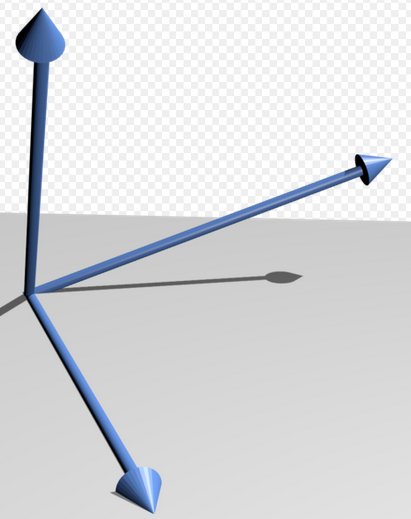
\includegraphics[width=.4\linewidth]{Independent.PNG}
	  \caption{Independent vectors}
	  \label{fig:sub1}
	\end{subfigure}%
	\begin{subfigure}{.5\textwidth}
	  \centering
	  
\includegraphics[width=.4\linewidth]{Dependent.PNG}
	  \caption{Dependent vectors}
	  \label{fig:sub2}
	\end{subfigure}
	\caption{Three vectors showing dependency}
	\label{fig:test}
\end{figure}
When solving a linear equation, the dependency of the matrix columns defines the number of
solutions. The three vectors either lie in a plane or they do not lie in a plane.
\begin{itemize}
	\item Independent vectors: $Ax=0$ has \textbf{one} solution. Matrix $A$ is invertible.
	\item Dependent vectors: $Ax=0$ has \textbf{many} solutions. Matrix $A$ is non-invertible.
\end{itemize}
\pagebreak
\subsection{Linear Equations}
Linear algebra solves a system of equations which are linear (Only multiplied by numbers). 
\par When a system of equations are expressed as $Ax=b$, matrix $A$ is called \textbf{Coefficient
Matrix}.
\par
Linear algebra can be viewed as Rows or Columns.
\begin{itemize}
	\item Row Picture: Shows two lines meeting at a single point (Solution)
	\begin{figure}[h!]
		\centering
		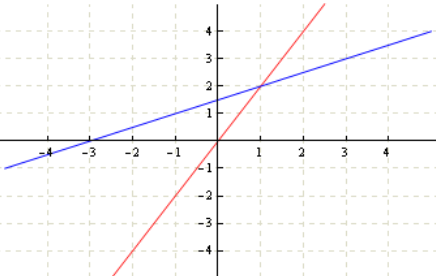
\includegraphics[scale=0.5]{Row.PNG}
		\caption{Row picture indicating the point where two lines meet}
		\label{}
	\end{figure}
	\item Column Picture: Combines the column vectors to produce a vector $b$
	\begin{figure}[h!]
		\centering
		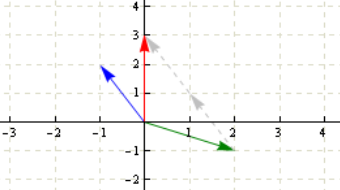
\includegraphics[scale=0.5]{Column.PNG}
		\caption{Column picture showing the resulting vector}
		\label{}
	\end{figure}
\end{itemize}

For example:
\begin{align*} 
	x + 2y + 3z &=  6 \\ 
	2x + 5y + 2z &=  4\\
	6x - 3y + z &= 2
\end{align*}
The system of equations can be viewed as follows:
\begin{itemize}
	\item Row: Three planes meeting at a single point
	\item Column: Three columns to produce a vector $b$
\end{itemize}
\pagebreak
\subsection{Elimination}
The elimination method is a way to solve linear equations where two unknowns are reduced to one
unknown in one of the equations. \par 
\begin{figure}[h!]
	\centering
	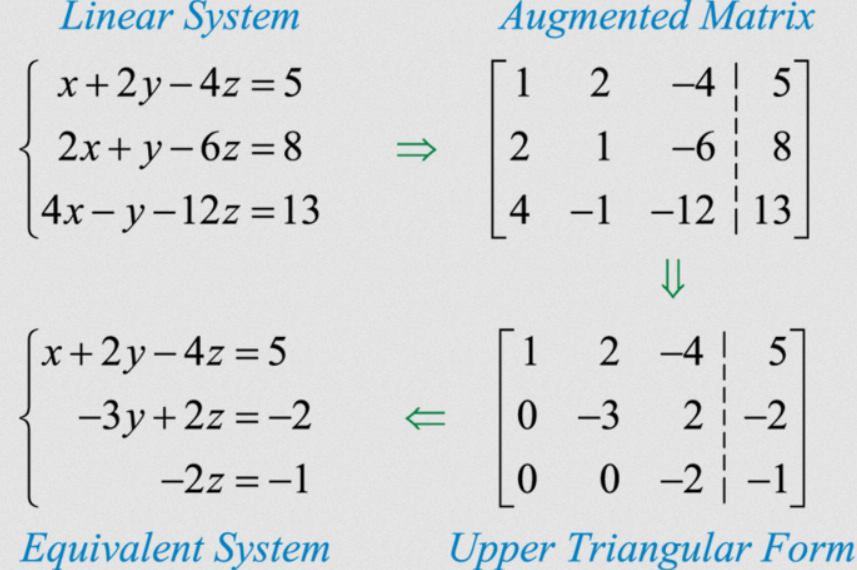
\includegraphics[scale=0.4]{Elimination.PNG}
	\caption{Process of Elimination obtaining one unknown to solve}
	\label{}
\end{figure}
The Elimination method produces a \textbf{Upper Triangular System} from which then system is solved
from bottom up (\textbf{Back Substitution}). \par 
Graphically, the point of intersection of lines do not change. \par 
Elimination method fails sometimes and could lead to three cases:
\begin{itemize}
	\item No solution
	\item Infinite solution
	\item Fixable by exchanging rows
\end{itemize}
\subsubsection{No solutions}
\begin{align*} 
	x - 2y &=  1 && x-2y =1\\ 
	3x - 6y &=  11 && 0y=8
\end{align*}
Graphically speaking:
\begin{itemize}
	\item Row Picture: This is two \textbf{parallel lines} that never cross hence there is never a
	solution.
	\item Column Picture: Columns do not combine to produce a third vector $b$ \ \footnote{Page 47 of Strang: Introduction to linear algebra}
\end{itemize} 
\subsubsection{Infinite solutions}
\begin{align*} 
	x - 2y &=  1 && x-2y =1\\ 
	3x - 6y &=  3 && 0y=0
\end{align*}
Graphically speaking:
\begin{itemize}
	\item Row Picture: This is two \textbf{parallel lines} that have become the same line. Every
	point on that line satisfies both line equations.
	\item Column Picture: Two columns become the same column and the vector $b$ is the same as the two initial vectors. \ \footnote{Page 47 of Strang: Introduction to linear algebra}
\end{itemize} 
\subsection{Matrix}
There are types of matrices:
\begin{itemize}
	\item Elimination matrix $E$: Subtracts/adds a multiple of a row to another row
	\item Identity matrix: Contains only 1 along the major diagonal
	\item Permutation matrix: Matrix containing information about row exchanges
	\item Augmented matrix: Matrix containing the Coefficient Matrix $A$ and right side $b$ matrix
	\item Zero matrix: A matrix containing 0 only
\end{itemize}
\subsubsection{Matrix operation rules}
Matrix multiplication:
$$\begin{bmatrix}
	m \\
	n 
	\end{bmatrix} * \begin{bmatrix}
		n \\
		p 
		\end{bmatrix} = 
		\begin{bmatrix}
			m \\
			p 
		\end{bmatrix} $$
To multiply matrices $A$ and $B$, $A$ has \textit{n} columns and $B$ must have \textit{n} rows.
\subsubsection{Matrix operation laws}
Addition laws:
\begin{itemize}
	\item Commutative law: $A+B=B+A$
	\item Distributive law: $c(A+B)=cA+cB$
	\item Associative law: $A+(B+C)=(A+B)+C$
\end{itemize}
Multiplication laws:
\begin{itemize}
	\item Commutative law: $AB\neg BA$
	\item Right Distributive law: (A+B)C=AC+BC
	\item Left Distributive law: C(A+B)=CA+CB
	\item Associative law: A(BC)=(AB)C 
\end{itemize}
\vfill
\pagebreak
\subsection{Inverse matrix}
Not all matrices have inverses. Matrix $A$ is invertible if there exists a matrix $A^{-1}$ which
$$A*A^{-1}=A^{-1}*A=I$$
Notes:
\begin{itemize}
	\item An invertible matrix cannot have a 0 determinant
	\item Inverse exists if elimination produces \textit{n} pivots (Same number of rows)
	\item There exists only one inverse for each matrix
	\item If there is a non-zero $x$ which $Ax=0$ then $A$ has no inverse - $x=A^{-1}*0$ is impossible
	\item $2\times 2$ matrix is invertible if $ad-bc$ is not 0
	\item The product $A\times B$ has an inverse if $A$ and $B$ each have their own inverses
\end{itemize}
Inverse matrices can be found by using the Gauss-Jordan method.
\subsection{Transposes and Permutations}
The rows and columns of a matrix are swapped. 
\begin{align*} 
	A &=  \begin{bmatrix}
		1&&2&&3 \\
		0&&0&&4
	\end{bmatrix} && A^{T}=\begin{bmatrix}
		1&&0 \\
		2&&0 \\
		3&&4 
	\end{bmatrix}
\end{align*}
Converting to transposes are handled differently during operations:
\begin{itemize}
	\item Sum: $A+B$ is $A^T + B^T$
	\item Product: $AB$ is $(AB)^T = B^T A^T$
	\item Inverse: $A^{-1}$ is $(A^{-1})^T = (A^T)^{-1}$
\end{itemize}
\pagebreak

\section{Vector Spaces and Subspaces}
There are three levels of understanding in Linear Algebra: Numbers, Vectors and Spaces. \par 
It is important to consider the \textbf{spaces} of vectors and their \textbf{subspaces}.
The most important vector spaces are $\textbf{R}^n$ where $n$ represents the number of components
within in a vector. This space consists of all column vectors with $n$ components.\par 
The two essential vector operations (Addition and Multiplication) occur inside the vector space to
produce linear combinations. 
\begin{tcolorbox}[breakable,colback=white,colframe=black,width=\dimexpr\textwidth+12mm\relax,enlarge left by=-6mm]
		\textit{Can add any vectors in $\textbf{R}^n$ and multiple any vector by any scalar. The results must \textbf{stay within the vector space} to satisfy the laws of the problem set.\footnote{Refer to page 121 of Strang Intro to Linear Algebra for the eight laws}}
\end{tcolorbox}
There are other vector spaces besides $\textbf{R}^n$:
\begin{itemize}
	\item $M$: Vector space of all real $2\times 2$ matrices
	\item $F$: Vector space of all real functions $f(x)$
	\item $Z$: Vector space consisting of only a zero vector. No space cannot exist without a zero
	vector, it is the smallest possible vector space. Hence, every vector space has a $Z$ vector space.
\end{itemize}
\subsection{Subspaces}
There are subspaces of $\textbf{R}^n$ that can be investigated. For example, in $\textbf{R}^3$
space, a plane through the origin or can be considered a vector space as well as $Z$. They exists
within the vector space of $\textbf{R}^3$. 
\begin{tcolorbox}[breakable,colback=white,colframe=black,width=\dimexpr\textwidth+12mm\relax,enlarge
left by=-6mm] 
	\textbf{Subspace}: A subset of a vector space (Including Zero Vector) that satisfies two
		requirements, where $v$ and $w$ are vectors in the subspace: 
		\begin{itemize}
			\item $v+w$ is in the subspace
			\item $c*v$ is in the subspace (where $c$ is a scalar)
		\end{itemize}
\end{tcolorbox}

For example the possible subspaces for $\textbf{R}^3$ are:
\begin{itemize}
	\item $L$ any lines through origin
	\item $P$ any plane through origin
	\item $Z$ single vector at origin
	\item $\textbf{R}^3$ whole space
\end{itemize}
\vfill{}
\subsection{Column space of A}
Linear algebra solves for $Ax=b$ and important subspaces are tied directly to matrix $A$. If $A$ is
not invertible then the system is solvable for \textit{some values of $b$}. The values that form the
possible matrix $b$ form the \textbf{column space} of A. \par 
In the system, values of $Ax$ and, as a result $b$ is defined by the possible combinations of the
columns of $A$. hence, to get all the values of $b$, all possible values of $x$ are used (All linear
combinations). \par 
This section has a relation to 'Independence'. Some columns/rows could be combinations
of others meaning that it would not span the entire $R^n$.
\begin{tcolorbox}[breakable,colback=white,colframe=black,width=\dimexpr\textwidth+12mm\relax,enlarge left by=-6mm]
\textbf{Column Space}: Consists of all linear combinations of the columns of $A$ to form all possible vectors
$Ax$. Forms the column space $C(A)$.
\end{tcolorbox}
This means that to solve $Ax=b$, $b$ has to be in the column space produced by $A$ or there is no
solution. \par 
\textbf{Example}: $A$ is $[m\times n]$ so its columns have $m$ components. The column space of $A$ is a
subspace of $R^m$. $Ax$ is defined as: 
$$\begin{bmatrix}
	1 & 0\\ 
	4 & 3\\ 
	2 & 3
	\end{bmatrix} * \begin{bmatrix}
		x_1 \\ 
		x_2
		\end{bmatrix} = x_1\begin{bmatrix}
			1\\ 
			4\\ 
			2
			\end{bmatrix} + x_2\begin{bmatrix}
				0\\ 
				3\\ 
				3
				\end{bmatrix}  $$
$b$ is defined as the linear combination of columns of $A$:
$$b=x_1\begin{bmatrix}
	1\\ 
	4\\ 
	2
	\end{bmatrix} + x_2\begin{bmatrix}
		0\\ 
		3\\ 
		3
		\end{bmatrix} $$
		The $b$ vector lies in the plane created by the two column vectors which is a subspace
		within the $R^3$ space.
\subsection{Nullspace of $A$}
The nullspace of $A$ is found by solving for $Ax=0$. The solutions form the nullspace of $A$ and are
denoted by $N(A)$. $x=0$ is always in the nullspace so every matrix $A$ has a nullspace.\par 
The solution vectors form the nullspace subspace when solving for ($Ax=0$ and $Ay=0$) - this is tested with two conditions:
\begin{itemize}
	\item $A(x+y)=0+0$
	\item $A(cx)=c0$
\end{itemize}
Any combinations made will remain in the nullspace hence it is a subspace. \par 
As previous, the matrix $A$ is defined by $[m\times n]$. When solving $Ax=0$, the vector $x$ are in
$R^n$, meaning the vector has $n$ components. \par 
\textbf{Example}: $x+2y+3z=0$ where $A = \begin{bmatrix}
	1 & 2 & 3
	\end{bmatrix}$ \par
The equation $Ax=0$ produces a plane through the origin. The plane is a subspace of $R^3$ - the
nullspace of $A$. \par 
To describe the nullspace of $A$, one point on the line (a \textbf{special solution}) is chosen. All
the points on the line are multiples of this special solution. It is important to sometimes realise
that rows in a matrix can be multiples of other rows - row picture: line of that row is the same
line as the other row, does not contribute anything to the picture.\par 
\textbf{Example}:
\begin{align} \nonumber
	x_1 + 2x_2 = 0 \\ 
	3x_1 + 6x_2 = 0 \nonumber
\end{align}
This can be simplified to:
\begin{align} \nonumber
	x_1 + 2x_2 = 0 \\
	0=0\nonumber
\end{align}
The nullspace of this system of equations can be found by choosing a special solution: let $x_2 =
1$. The nullspace consists of all combinations of special solutions:
$$Nullspace = \begin{bmatrix}
	-2 \\ 
	1
\end{bmatrix}$$
There could be more than one special solution. For example:
$$x+2y+3z=0$$
\begin{center}
	$\begin{bmatrix}
		1 & 2 & 3
	\end{bmatrix} * \begin{bmatrix}
		x \\ 
		y \\
		z
	\end{bmatrix} = 0$ has special solutions $s_1 = \begin{bmatrix}
		-2 \\ 
		1 \\
		0
	\end{bmatrix}$ and $s_2 = \begin{bmatrix}
		-3 \\ 
		0 \\
		1
	\end{bmatrix}$
\end{center}
The \textit{free components} are usually set to 1 or 0. \textit{Free Components} are columns
without a pivot which is column 2 and 3 in the above equation. The resulting matrix can be further
simplified by finding \textit{Reduced Form: R}.
\subsubsection{Process to finding Nullspace}
Elimination is required to simplify $A$ by row operations before solutions can be obtained. The two
stages:
\begin{itemize}
	\item Forward Elimination: Convert $A$ to Upper Triangular $U$ (Echelon Form)
	\item Back Substitution: Produces $x$ from $Ux$
\end{itemize}
In Forward Elimination, the difference is that some pivots encountered will be 0. The process simply continues to the next column until
the process is completed. \par 
\textbf{Example}:
\begin{center}
	$A=\begin{bmatrix}
		1&1&2&3 \\ 
		2&2&8&10 \\
		3&3&10&13
	\end{bmatrix}$ \par 
\end{center}
Column 2 is a 0 pivot:
\begin{center}
	$A=\begin{bmatrix}
		1&1&2&3 \\ 
		0&\textbf{0}&4&4 \\
		0&0&4&4
	\end{bmatrix}$
\end{center}
Moving to next 'pivot' point and continue: 
\begin{center}
	$A=\begin{bmatrix}
		1&1&2&3 \\ 
		0&0&4&4 \\
		0&0&\textbf{0}&0
	\end{bmatrix}$
\end{center}
At the end of Forward Elimination, row 2 and row 3 are the same hence row 3 does not contribute to
the picture. The 'Echelon Form' is found and the following can be identified:
\begin{itemize}
	\item Pivot Columns: $x_1$ and $x_3$
	\item Free Columns (No pivots): $x_2$ and $x_4$
	\item Rank (Number of Pivot Columns - equations that contributed): 2
\end{itemize}
\begin{tcolorbox}[breakable,colback=white,colframe=black,width=\dimexpr\textwidth+12mm\relax,enlarge left by=-6mm]
	If a matrix is invertible, there will be \textbf{no free pivots}. All variables are pivot variables.
\end{tcolorbox}
In Back Substitution, the Free Columns are substituted with 1s and 0s to obtain Special Solutions.
The number of Special Solutions are determined by the number of Free Columns. \par 
After finding the values of Free Columns, these are combined to form the complete solution denoted as:
\begin{center}
	$x=x_2*\begin{bmatrix}
		-1 \\ 
		1 \\
		0 \\
		0
	\end{bmatrix} + x_4*\begin{bmatrix}
		-1 \\ 
		0 \\
		-1 \\
		1
	\end{bmatrix} = \begin{bmatrix}
		-x_2 - x_4 \\ 
		x_2 \\
		-x_4 \\
		x_4
	\end{bmatrix} $
\end{center}
\begin{tcolorbox}[breakable,colback=white,colframe=black,width=\dimexpr\textwidth+12mm\relax,enlarge left by=-6mm]
Summary of steps to find the nullspace of $A$:
\begin{enumerate}
	\item Obtain Echelon Form through Elimination
	\item Identify: Pivot Columns and Free Columns
	\item Set first free column variable equal to 1 and the others to 0
	\item Find corresponding values from the equation created
	\item Repeat for each Free Column identified
	\item The resulting linear combinations are the nullspace
\end{enumerate}
\end{tcolorbox}

\subsection{Echelon Matrices}
An echelon matrix is a matrix form as the result of Gaussian Elimination.
\begin{center}
		$U=\begin{bmatrix} 
			p&x&x&x&x&x&x \\ 
			0&p&x&x&x&x&x \\
			0&0&0&0&0&p&x \\
			0&0&0&0&0&0&0
		\end{bmatrix}$ 
		\begin{itemize}
			\item Three Pivot Variables: $x_1$, $x_2$, $x_6$
			\item Four Free Variables: $x_3$, $x_4$, $x_5$, $x_7$
			\item Four Special Solutions
		\end{itemize}
\end{center}
To repeat, the Column Space is a subspace of $R^4$ and Nullspace is a subspace of $R^7$. The
dimension of the nullspace is the number of free variables, 4 in this case.

\subsection{Reduced Row Echelon Matrix: $R$}
Provided the Echelon Matrix: 
$$U=\begin{bmatrix}
	1&1&2&3 \\
	0&0&4&4 \\
	0&0&0&0
\end{bmatrix}$$
The Reduced Row Echelon Matrix has 0's above and below the pivots, and 1's as pivots.
\begin{center}
	Divide row 2 by 4 and subtract rows: \par $R=rref(A)=\begin{bmatrix}
		1&1&0&1 \\
		0&0&1&1 \\
		0&0&0&0
	\end{bmatrix}$
\end{center}
Reduced Row Echelon Form makes it easy to find special solutions.
\begin{itemize}
	\item Set $x_2=1$ and $x_4=0$. Solve.
	\item Set $x_2=0$ and $x_4=1$. Solve.
\end{itemize}
\begin{tcolorbox}[breakable,colback=white,colframe=black,width=\dimexpr\textwidth+12mm\relax,enlarge left by=-6mm]
If the matrix is invertible, the Reduced Row Echelon matrix is the identity matrix. 
\end{tcolorbox}
\pagebreak
\subsection{The Rank and Row Reduced Form}
The size of the matrix is given by $m$ and $n$ but it is not the true size of the linear system. The
true size of the Matrix $A$ is determined by its rank - the number of pivots $r$. This is due to
eliminations like columns or rows that are multiples or a combination of rows - these will all
reduce to 0s in the Reduced Row Echelon form. \par
\begin{tcolorbox}[breakable,colback=white,colframe=black,width=\dimexpr\textwidth+12mm\relax,enlarge left by=-6mm]
Every free columns \textbf{are} combinations of earlier pivot columns. \\
Every pivot columns \textbf{are not} combinations of earlier pivot columns. 
\end{tcolorbox}
\textbf{Example}: Given the matrix $A=\left (\begin{matrix}
	1 & 1 & 2 & 4\\ 
	1 & 2 & 2 & 5\\ 
	1 & 3 & 2 & 6\\ 
   \end{matrix}  \right )$
   \begin{itemize}
	   \item Column 1 and 2 are going in different directions.
	   \item Column 2 is the multiple of Column 3.
	   \item Column 4 is the addition of Column 1, 2 and 3.
   \end{itemize}
   The matrix will only have 2 pivots and 2 free column.
   \begin{itemize}
	   \item Find the Upper Triangular form: 
	   \begin{align*}
        U & = \left (\begin{matrix}
			1 & 1 & 2 & 4\\ 
			1 & 2 & 2 & 5\\ 
			1 & 3 & 2 & 6\\ 
		   \end{matrix}  \right ) \\
		  & = \left (\begin{matrix}
			1 & 1 & 2 & 4\\ 
			0 & 1 & 0 & 1\\ 
			0 & 2 & 0 & 2\\ 
		   \end{matrix}  \right ) \\
		  & = \left (\begin{matrix}
			1 & 1 & 2 & 4\\ 
			0 & 1 & 0 & 1\\ 
			0 & 0 & 0 & 0\\ 
		   \end{matrix}  \right )
	\end{align*}
	\item Find the Reduced Row Echelon $R$ form:
	\begin{align*}
        R & = \left (\begin{matrix}
			1 & 0 & 2 & 3\\ 
			0 & 1 & 0 & 1\\ 
			0 & 0 & 0 & 0\\ 
		   \end{matrix}  \right )
	\end{align*}
   \end{itemize}
   \subsubsection{Rank One}
   \subsubsection{Pivot Columns}
   Pivot columns consists of 1's in pivots and 0's in the rest.
   \subsubsection{Special Solutions}
   Each special solutions has one variable set to 1 and the other variables to 0. There is a special
   solution for every free variable.
   \begin{tcolorbox}[breakable,colback=white,colframe=black,width=\dimexpr\textwidth+12mm\relax,enlarge left by=-6mm]
   $Ax=0$ has $r$ pivots and $n-r$ free variables. The nullspace matrix $N$ contains $n-r$ special
   solutions.
   \end{tcolorbox}
   Special solutions are easily identified with $R$. The $R$ format is simplified into:
   $$N=\begin{bmatrix}
	-F\\ 
	I
	\end{bmatrix}$$ where $I$ is defined by $n-r$ and F is defined by $r$. \par 
	\textbf{Example:} Given the special solutions: $Rx=x_1+2x_2+3x_3=0$
	
	\noindent\begin{minipage}{.5\linewidth}
	\begin{equation*}
	  R = \begin{bmatrix}
		1 && 2&&3
		\end{bmatrix}
	\end{equation*}
	\end{minipage}%
	\begin{minipage}{.5\linewidth}
	\begin{equation*}
		N = \begin{bmatrix}
			-F \\
			I
			\end{bmatrix} = 
			\begin{bmatrix}
			-2 && -3 \\
			1 && 0 \\
			0 && 1
			\end{bmatrix}
	\end{equation*}
	\end{minipage} 
	\\
	The rank is one. The special solutions are $(-2, 1, 0)$ and ($-3, 0, 1)$.
	\pagebreak
	\subsection{The Complete Solution to $Ax=b$}
	\subsubsection{Solvability of $Ax=b$}
	The existence of solutions to $Ax=b$ needs to be established first. There is always a solution
	to $Ax=0$ but there is not always a solution to $Ax=b$ - $b$ needs to be in the column space
	($C(A)$). 
	\par 
	\begin{tcolorbox}[breakable,colback=white,colframe=black,width=\dimexpr\textwidth+12mm\relax,enlarge left by=-6mm]
	The process for checking for solvability is:
	\begin{enumerate}
		\item Form Augmented Matrix
		\item Elimination process
		\item Last row indicates condition required for solvability (Solvability Condition)
		\begin{itemize}
			\item Consistent: Last row is all 0's and has a solution
			\item Inconsistent: Last row is not all 0's and has no solution
		\end{itemize}
	\end{enumerate}
	\end{tcolorbox}
	\textbf{Example:} Given the matrix: 
	\begin{equation*}
		A =\begin{bmatrix}
			1 & 2 & 2 & 2 \\
			2 & 4 & 6 & 8 \\
			3 & 6 & 8 & 10
			\end{bmatrix}
	\end{equation*}
	Going through the process listed above: 
	\begin{center}
		$A=
	\begin{bmatrix}
	1 & 2 & 2 & 2 &  |& b_1\\ 
	2 & 4 & 6 &  8&  |& b_2\\ 
	3 & 6 & 8 &  10&|  & b_3
	\end{bmatrix} 
	\xrightarrow[\substack{R_2 - 2R_1 \\ R_3 - 3R_1}]{}
	\begin{bmatrix}
	1 & 2 & 2 & 2 & | & b_1\\ 
	0 & 0 & 2 & 4 & | & b_2-2b_1\\ 
	0 & 0 & 2 & 4 & | & b_3-3b_1
	\end{bmatrix} 
	\xrightarrow[\substack{R_3 - R_2}]{}
	\begin{bmatrix}
	1 & 2 & 2 & 2 & | & b_1\\ 
	0 & 0 & 2 & 4 & | & b_2-2b_1\\ 
	0 & 0 & 0 & 0 & | & b_3-b_2-b_1
	\end{bmatrix} $
	\end{center}
	
	The last row equation indicates solutions exists only if:
	$b_3+b_2+b_1=0$

	\subsubsection{Finding the Complete Solution}
	The complete solution $Ax=b$ is composed of: \par 
	\begin{center}
		$x = x_p$ (Particular solution) $+ x_n$ (Other
	solutions in nullspace.)
	\end{center}
	As mentioned previously, complete solution is defined as: $x=x_p + x_n$ where:
	\begin{itemize}
		\item $x_{particular}$: Solves for $Ax_p=b$
		\item $x_{nullspace}$: Solves for $Ax_n=0$
	\end{itemize}
	\begin{tcolorbox}[breakable,colback=white,colframe=black,width=\dimexpr\textwidth+12mm\relax,enlarge left by=-6mm]
		Summary of steps to find the complete solution of A:
	\begin{enumerate}
		\item Find 'Echelon Form' of \textbf{Augmented Coefficient Matrix}
		\item Establish if system is solvable
		\item Solve Homogenous Equation $Ax=0$ for nullspace
		\item Find Particular Solution $Ax=b$: $x_p$
		\item Solution is the combination of Particular Solution and Nullspace Solution
	\end{enumerate}
	\end{tcolorbox}
	\textbf{Example}: Given $\begin{bmatrix}
		1 & 2 & 2 & 2 \\ 
		2 & 4 & 6 & 8 \\ 
		3 & 6 & 8 & 10
		\end{bmatrix}*\textbf{\underbar{x}} = \begin{bmatrix}
		1\\ 
		5\\ 
		6
		\end{bmatrix}$ solve. \par 
		Augmented matrix in Echelon form:
		$$[A:\underbar{b}]\sim
		\begin{bmatrix}
			\textbf{1} & 2 & 2 & 2 & | & 1\\ 
			0 & 0 & \textbf{2} & 4 & | & 3\\ 
			0 & 0 & 0 & 0 & | & 0
		\end{bmatrix}$$
		Finding the Nullspace Solution by setting Free Column Variables to 1's and 0's
		$$x_n = p*
		\begin{bmatrix}
			-2 \\ 
			1  \\ 
			0 \\
			0
		\end{bmatrix}+ q*\begin{bmatrix}
			2 \\ 
			0  \\ 
			-2 \\
			1
		\end{bmatrix}$$ 
		The Particular Solution is found with Free Column Variables all set to 0
		$$x_p = 
		\begin{bmatrix}
			-2 \\ 
			0  \\ 
			\frac{3}{2} \\
			0
		\end{bmatrix}$$ 
		The complete solution is: 
		$$\underbar{x} = 
		\begin{bmatrix}
			-2 \\ 
			0  \\ 
			\frac{3}{2} \\
			0
		\end{bmatrix} +
		p*
		\begin{bmatrix}
			-2 \\ 
			1  \\ 
			0 \\
			0
		\end{bmatrix}+ q*\begin{bmatrix}
			2 \\ 
			0  \\ 
			-2 \\
			1
		\end{bmatrix}$$ 

		\begin{tcolorbox}[breakable,colback=white,colframe=black,width=\dimexpr\textwidth+12mm\relax,enlarge left by=-6mm]
			Summary:
			\begin{itemize}
				\item Elimination on $\begin{bmatrix}
					A & b
					\end{bmatrix}$ leads to 
					$\begin{bmatrix}
						R & d
					\end{bmatrix}$. This means $Ax=b$ is equal to $Rx=d$.
				\item $Ax=b$ and $Rx=d$ are solvable only if rows in $R$ with 0s also have 0s in $d$.
				\item When $Rx=d$ is solvable, one \textit{particular solution: $x_p$ has all free variable
				equal to zero.}
			\end{itemize}
		\end{tcolorbox}

%%%%%%%%%%%%%%%%%%%%%%%%%%%%%%%%%%%%%%%%%%%%%%%%%%%%%%%%%%%%%%%%%%%%%%%%%%%%%%%%%%%%%%%%%%%%%%%%%%%%%%%%%%
\end{document}
